\documentclass[floatsintext,man]{apa6}

\usepackage{amssymb,amsmath}
\usepackage{ifxetex,ifluatex}
\usepackage{fixltx2e} % provides \textsubscript
\ifnum 0\ifxetex 1\fi\ifluatex 1\fi=0 % if pdftex
  \usepackage[T1]{fontenc}
  \usepackage[utf8]{inputenc}
\else % if luatex or xelatex
  \ifxetex
    \usepackage{mathspec}
    \usepackage{xltxtra,xunicode}
  \else
    \usepackage{fontspec}
  \fi
  \defaultfontfeatures{Mapping=tex-text,Scale=MatchLowercase}
  \newcommand{\euro}{€}
\fi
% use upquote if available, for straight quotes in verbatim environments
\IfFileExists{upquote.sty}{\usepackage{upquote}}{}
% use microtype if available
\IfFileExists{microtype.sty}{\usepackage{microtype}}{}

% Table formatting
\usepackage{longtable, booktabs}
\usepackage{lscape}
% \usepackage[counterclockwise]{rotating}   % Landscape page setup for large tables
\usepackage{multirow}		% Table styling
\usepackage{tabularx}		% Control Column width
\usepackage[flushleft]{threeparttable}	% Allows for three part tables with a specified notes section
\usepackage{threeparttablex}            % Lets threeparttable work with longtable

% Create new environments so endfloat can handle them
% \newenvironment{ltable}
%   {\begin{landscape}\begin{center}\begin{threeparttable}}
%   {\end{threeparttable}\end{center}\end{landscape}}

\newenvironment{lltable}
  {\begin{landscape}\begin{center}\begin{ThreePartTable}}
  {\end{ThreePartTable}\end{center}\end{landscape}}




% The following enables adjusting longtable caption width to table width
% Solution found at http://golatex.de/longtable-mit-caption-so-breit-wie-die-tabelle-t15767.html
\makeatletter
\newcommand\LastLTentrywidth{1em}
\newlength\longtablewidth
\setlength{\longtablewidth}{1in}
\newcommand\getlongtablewidth{%
 \begingroup
  \ifcsname LT@\roman{LT@tables}\endcsname
  \global\longtablewidth=0pt
  \renewcommand\LT@entry[2]{\global\advance\longtablewidth by ##2\relax\gdef\LastLTentrywidth{##2}}%
  \@nameuse{LT@\roman{LT@tables}}%
  \fi
\endgroup}


  \usepackage{graphicx}
  \makeatletter
  \def\maxwidth{\ifdim\Gin@nat@width>\linewidth\linewidth\else\Gin@nat@width\fi}
  \def\maxheight{\ifdim\Gin@nat@height>\textheight\textheight\else\Gin@nat@height\fi}
  \makeatother
  % Scale images if necessary, so that they will not overflow the page
  % margins by default, and it is still possible to overwrite the defaults
  % using explicit options in \includegraphics[width, height, ...]{}
  \setkeys{Gin}{width=\maxwidth,height=\maxheight,keepaspectratio}
\ifxetex
  \usepackage[setpagesize=false, % page size defined by xetex
              unicode=false, % unicode breaks when used with xetex
              xetex]{hyperref}
\else
  \usepackage[unicode=true]{hyperref}
\fi
\hypersetup{breaklinks=true,
            pdfauthor={},
            pdftitle={Early language experience in a Papuan village},
            colorlinks=true,
            citecolor=blue,
            urlcolor=blue,
            linkcolor=black,
            pdfborder={0 0 0}}
\urlstyle{same}  % don't use monospace font for urls

\setlength{\parindent}{0pt}
%\setlength{\parskip}{0pt plus 0pt minus 0pt}

\setlength{\emergencystretch}{3em}  % prevent overfull lines


% Manuscript styling
\captionsetup{font=singlespacing,justification=justified}
\usepackage{csquotes}
\usepackage{upgreek}

 % Line numbering
  \usepackage{lineno}
  \linenumbers


\usepackage{tikz} % Variable definition to generate author note

% fix for \tightlist problem in pandoc 1.14
\providecommand{\tightlist}{%
  \setlength{\itemsep}{0pt}\setlength{\parskip}{0pt}}

% Essential manuscript parts
  \title{Early language experience in a Papuan village}

  \shorttitle{Early language experience in a Papuan village}


  \author{Marisa Casillas\textsuperscript{1}, Penelope Brown\textsuperscript{1}, \& Stephen C. Levinson\textsuperscript{1}}

  % \def\affdep{{"", "", ""}}%
  % \def\affcity{{"", "", ""}}%

  \affiliation{
    \vspace{0.5cm}
          \textsuperscript{1} Max Planck Institute for Psycholinguistics  }

  \authornote{
    Correspondence concerning this article should be addressed to Marisa
    Casillas, P.O. Box 310, 6500 AH Nijmegen, The Netherlands. E-mail:
    \href{mailto:Marisa.Casillas@mpi.nl}{\nolinkurl{Marisa.Casillas@mpi.nl}}
  }


  \abstract{To be completed later.}
  \keywords{Child-directed speech, linguistic input, non-WEIRD, vocal maturity, turn
taking, interaction, Papuan \\

    \indent Word count: XXXXX (XXXX not including references)
  }





\usepackage{amsthm}
\newtheorem{theorem}{Theorem}[section]
\newtheorem{lemma}{Lemma}[section]
\theoremstyle{definition}
\newtheorem{definition}{Definition}[section]
\newtheorem{corollary}{Corollary}[section]
\newtheorem{proposition}{Proposition}[section]
\theoremstyle{definition}
\newtheorem{example}{Example}[section]
\theoremstyle{definition}
\newtheorem{exercise}{Exercise}[section]
\theoremstyle{remark}
\newtheorem*{remark}{Remark}
\newtheorem*{solution}{Solution}
\begin{document}

\maketitle

\setcounter{secnumdepth}{0}



\section{Introduction}\label{intro}

There is mounting evidence that children in many parts of the world
typically acquire their language(s) with little direct speech from
adults in the first few years of life. Indeed, recent studies that have
directly measured the quantity of speech addressed to children under age
five across a number of indigenous communities in southern Mexico
(Shneidman \& Goldin-Meadow, 2012; Casillas et al., forth), Bolivia
(Cristia et al., 2017; Cychosz et al., in prep; Scaff et al., in prep),
and northeastern Africa (Mastin et al., ??) have found that speech
directly addressed to young children is infrequent. The quantitative
findings of this work have, by and large, reinforced ethnographic
descriptions of these and other small-scale non-Western communities
(e.g., Ochs \& Schieffelin, Brown, etc.). Moreover, recent work applying
these techniques with North American children suggests that, even
Western middle-class contexts, the quantity of directed speech to
children is typically low: around 5--6 minutes per hour. How, then, do
children manage to accumulate sufficient lingusitic evidence from other
parts of their speech environment such that they become competent adult
language users?

Despite the linguistically and culturally diverse language environments
of the human past and present, children---no matter where they grow
up---typically learn the set of linguistic structures and patterns of
language use relevant to their community such that they are able to pass
on these learnable skills to the next generation without any explicit or
universal framework for teaching or learning. And while young language
learners do effect change on the lingusitic system they are learning
(e.g., NSL, creoles, etc., REFS), they tend to learn the language of
their parents and peers with high fidelity (REFS). However, this robust
ability to transmit languages across generations does not preculde the
possibility that there is meaningful variation in individual language
skill and individual language-learning trajectories.

Indeed, work focused on children growing up in (primarily) Western
societies has shown convincingly that environmental effects can
significantly impact children's language development: children who hear
\emph{more} and \emph{more pedagogical} speech in their day-to-day lives
(e.g., interactive book reading) show larger, faster-growing
vocabularies, faster lexical retrieval, and possibly even earlier use of
some morphosyntactic structures (REFS), with these different language
measures typically intercorrelated (REFS). Additional evidence comes
from children who are learning two or more languages, whose early
vocabulary development is impacted by how much speech they hear in each
language (Hoff REFS). In sum, while language learning on the scale of
whole generations is robust, there is noticeable sensitivity to the
precise language environment in which children find themselves,
particularly with respect to their vocabulary development.

This apparent paradox dissolves when we consider that some individual
language skills may be more directly sensitive to environmental input
(e.g., vocabulary size is increased by exposure to more words and word
types) while other language skills are either highly robust (e.g., early
categorical discrimination of sounds, the emergence of canonical
babbling) or only indirectly affected by environmental input (e.g.,
mastery of frequent syntactic structures--I NEED A CLEARER EXAMPLE
HERE). The mapping between sensitivity to experience and linguistic
skills opens up the possibility for both theoretical and applied
advances. Theoretically, this mapping sheds light on the phylogenetic
roots of language. In modern application, it directs efforts at
developmental intervention (e.g., in cases of clinical language delay)
towards behaviors that could conceivably be altered by a change in
environment.

Part and parcel of exploring sensitivity to the speech environment is
sketching out the cognitive toolkit that chilren may draw upon in
inferring linguistic structure from what they see and hear. Consider
that apparent robustness to environmental variation can come from
multiple cognitive scenarios. On the one hand, robustness may appear in
learning because of quasi-preprogrammed maturational factors (e.g., the
onset of pointing). On the other, it may appear because there are
several strategies children can rely on to extract information (e.g.,
attention to direct vs.~overhearable speech). Identifying and
investigating these individual mechanisms will be a crucial aspect of
better understanding the human language learning ability.

By systematically leveraging cross-cultural variation in children's
language environments we can make progress on both fronts: (a) testing
existing ideas about what linguistic skills are and aren't sensitive to
linguistic experience on previously-untested populations and (b)
identifying and testing alternative mechanisms that may help explain the
(lack of) variation in language skills observed, despite large
differences in linguistic environments.

In the current paper we describe the language-learning environment of
children growing up on Rossel Island, with a population of approximately
7000 people approximately 250 nautical miles off the south-east coast of
Papua New Guinea. we chose to investigate language learning on Rossel
Island for two reasons. First, prior ethnographic research has
demonstrated that adult interactions with young children are often
highly positively affective and intensely interactive in a face-to-face
context, much like the prototype of interaction with young children in a
Western context (Brown). On the other hand, reviews of prior work have
suggested that child-directed speech in small-scale indigenous
communities of this type has been found to be infrequent in most
communities studied so far (e.g., ALEX??) and so frequent intensive CDS
would be a rare opportunity to look at how this kind of a speech
environment influences learning in a different language. Second, the
language itself is elaborate in its morphosyntax and contains rare
phonological features, setting it up as an excellent \enquote{different}
language on which current theories about the trajectory of early
language development can be tested.

\subsection{The community}\label{the-community}

Yélî Dnye is a language spoken by approximately 5000 people, nearly all
of whom reside on Rossel Island, a remote island 250 nautical miles off
the mainland coast in Milne Bay Province, Papua New Guinea. While all
the neighboring languages fall into the Austronesian family, Rossel is a
presumed-Papuan isolate that features a phonological inventory and set
of grammatical features that are completely unattested in other
languages of the region. Partly due to its remoteness, most children on
Rossel Island grow up speaking it monolingually at home, only beginning
to learn English (the official lingua franca of Milne Bay Province) as
they progress through school, which typically begins when a child is 7
or 8 years old.

We were interested to investigate the language environment of children
acquiring Yélî Dnye because prior ethnographic work had suggested that
child-directed speech is highly frequent in this community, from mothers
and other adult caregivers, but also from other children. Therefore we
were interested in understanding how children's input environment
influenced their acquisition of this language with all its rare
structures.

However, to our surprise we found that Yélî children were not spoken to
very often at all. In fact, they were spoken to less often than the
Tseltal children we have studied in other work, who are growing up in a
community where children are indeed reportedly spoken to infrequently.

Then two interesting issues arise. First, is it the quality of short
interactions that give us an impression of quantity---should we abandon
this assumption? Maybe we weren't even aware of it. Second, is it the
quality of these short interactions that influences early language
learning?

\section{Method}\label{method}

This study was completed as part of a larger comparative project on
children's speech environments and linguistic development at two sites:
a Tseltal Mayan community in southern Mexico and this Rossel Island
community. Therefore all methods for annotation and analysis in this
study parallel those reported elsewhere for Tseltal Mayan children's
speech environments (Casillas, Brown, \& Levinson, forthcoming).

The data we present come from 7--9-hour recordings of a waking day at
home for the child. Children wore the recording device, which was an
elastic vest with a small stereo audio recorder across the chest
(Olympus WS-832 or WS-853) and a small camera that captured photos of
the child's frontal view at a fixed interval (every 15 seconds;
Narrative Clip 1). The camera was additionally outfitted with a fisheye
lens that, while distorting the images, allowed us to capture 180
degrees of children's frontal view. Because the camera and recorder are
separate devices, they were synched by means of a single, external watch
that was used to record the current time at start of recording on each
device individually, with accuracy down to the second (photographed by
the camera and spoken into the recorder). The photos are timestamped by
the camera such that the precise intervals between photos are captured.
These timestamps can be used with the cross-device time synchronization
cue to create photo-linked audio files of each recording, which are
formatted as videos (see urlrefs for scripts and more information). We
chose to make long-format recordings of children's language experience
at home to capture a range of different activity contexts and
interlocutors at different times of day (REFS). Previous work
investigating the trade-offs of short- versus long-format recordings of
parental speech have demonstrated that the apparent quantity of speech
children hear and some of the characteristics of that speech differs
depending on recording duration (day-by-day tamislemonda REFS). However,
short recordings often have the benefit of video data, which enables the
analyst to take visual information into account in transcribing and
interpreting the communicative behaviors captured. Those using daylong
recording methods instead have traditionally had to sacrifice this
visual context because of (current) technological limitations; there are
no miniature, lightweight (e.g., 400g; 5cm x 5cm or less) video
recorders on the market that can record for 7--16 hours. We aimed to
generate generalizable baseline estimates of how much speech children
hear in this community but wanted to maintain visual information for
later transcription and interpretation, leading to us developing this
novel daylong recording method (see also Abels REFS).

We used this technique to create daylong recordings of 57 children under
age 4;0 on Rossel Island in 2016 (Casillas et al HB), selecting 10
representative children between ages 0;0 and 3;0 for transcription and
analysis in the current study. The 10 children were selected to be
spread between the target age range (0;0--3;0) while also representing a
range of typical maternal education levels found in the community and
while being evenly split between male and female children (see also
ACLEW REFS). For each child we then selected a series of
non-overalapping sub-clips from the day for transription in the
following order: nine randomly-selected 2.5-minute clips, five
manually-selected \enquote{peak} turn-taking activity 1-minute clips,
five manually-selected \enquote{peak} vocal activity 1-minute clips, and
one 5-minute expansion of the best one-minute clip, for a total of 37.5
minutes of transcribed audio for each child (6.25 audio hours in total).
The criteria for manual clip selection are identical to those described
for the parallel study on Tseltal by Casillas and colleagues
(forthcoming).

We were limited to selecting sub-clips from 10 children for analysis
because of the time-intensive nature of transcribing these naturalistic
data; 1 minute of audio typically takes 60--70 minutes of time to be
segmented into utterances, transcribed, annotated, and loosely
translated into English (\textasciitilde{}400 hours). Given that Yélî
Dnye is nearly exclusively spoken on Rossel Island, where here is no
electricity and unreliable cell network coverage, transcription could
only be completed over the course of three 4--6 week visits by our
research group to the island in 2016, 2018, and 2019.

\begin{table}[tbp]
\begin{center}
\begin{threeparttable}
\caption{\label{tab:tab1}Demographic overview of the 10 children whose recordings are sampled in the current study, including from left to right: child's age (years;months.days); child's sex (M/F); mother's age (years); level of maternal education (none/primary/secondary/preparatory/university); and the number of people living in the child's household.}
\begin{tabular}{lllll}
\toprule
Age & \multicolumn{1}{c}{Sex} & \multicolumn{1}{c}{Mother's age} & \multicolumn{1}{c}{Level of maternal education} & \multicolumn{1}{c}{People in household}\\
\midrule
01m;09d & F & 31 & secondary & 8\\
03m;19d & M & 37 & primary & 9\\
04m;13d & M & 24 & preparatory & 5\\
07m;18d & M & 24 & secondary & 5\\
09m;03d & F & 29 & secondary & 5\\
12m;29d & F & 30 & primary & 9\\
16m;29d & M & 25 & secondary & 6\\
20m;03d & F & 33 & primary & 9\\
25m;22d & F & 21 & secondary & 4\\
35m;29d & M & 41 & primary & 8\\
\bottomrule
\end{tabular}
\end{threeparttable}
\end{center}
\end{table}

\begin{figure}
\centering
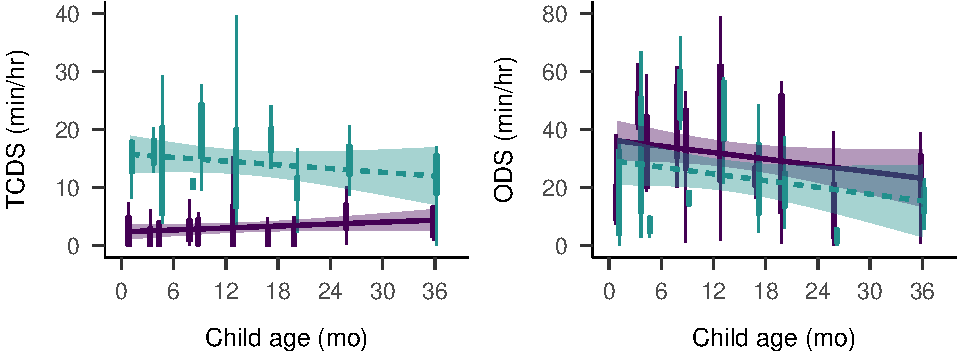
\includegraphics{Yeli-CLE_files/figure-latex/fig2-1.pdf}
\caption{\label{fig:fig2}Recording duration (black line) and sampled clips
(colored boxes) for each of the 10 recordings analyzed, sorted by child
age in months.}
\end{figure}

\begin{verbatim}
## pdf 
##   2
\end{verbatim}

\begin{verbatim}
## pdf 
##   2
\end{verbatim}

\begin{verbatim}
## pdf 
##   2
\end{verbatim}

\begin{verbatim}
## pdf 
##   2
\end{verbatim}

\begin{figure}
\centering
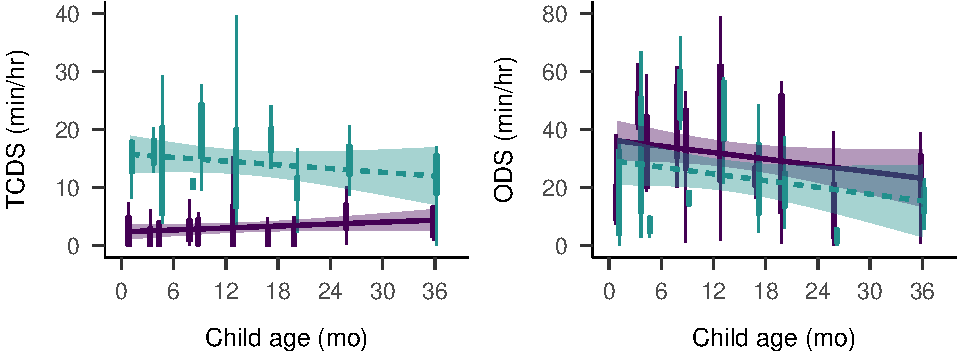
\includegraphics{Yeli-CLE_files/figure-latex/fig3-1.pdf}
\caption{\label{fig:fig3}Estimates of TCDS min/hr (left) and ODS min/hr
(right) across the sampled age range. Each box plot summarizes the data
for one child from the randomly sampled clips (purple; solid) or the
turn taking clips (green; dashed). Bands on the linear trends show 95\%
confidence intervals.}
\end{figure}

\begin{figure}
\centering
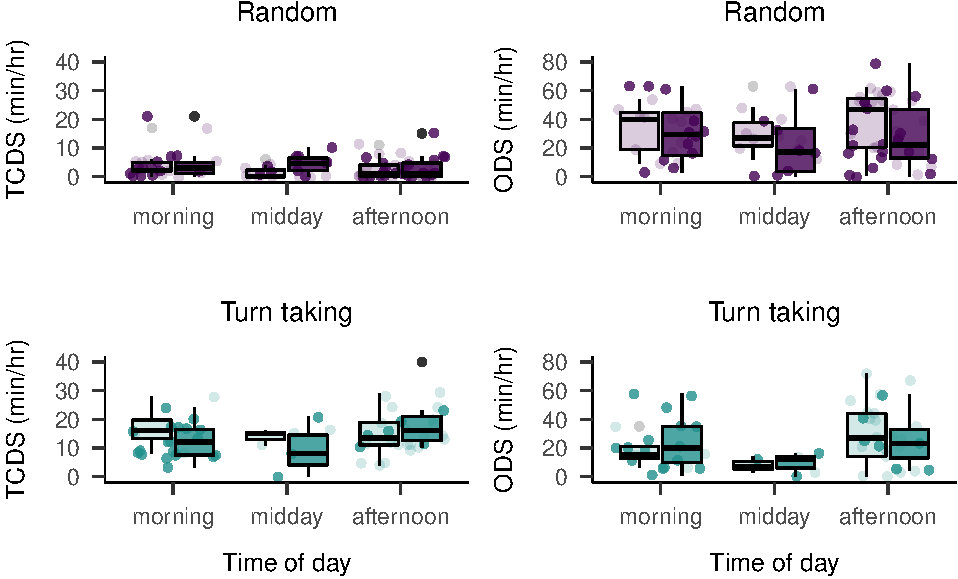
\includegraphics{Yeli-CLE_files/figure-latex/fig5-1.pdf}
\caption{\label{fig:fig5}Estimates of TCDS min/hr (left panels) and ODS
min/hr (right panels) across the recorded day in the random clips (top
panels) and turn-taking (bottom panels) clips. Each box plot summarizes
the data for children age 1;0 and younger (light) or age 1;0 and older
(dark) at the given time of day.}
\end{figure}

\begin{verbatim}
## [1] 3.13
\end{verbatim}

\begin{verbatim}
## [1] 2.95
\end{verbatim}

\begin{verbatim}
## [1] 1.58
\end{verbatim}

\begin{verbatim}
## [1] 6.26
\end{verbatim}

\begin{verbatim}
## [1] 14.62
\end{verbatim}

\begin{verbatim}
## [1] 15.07
\end{verbatim}

\begin{verbatim}
## [1] 10.39
\end{verbatim}

\begin{verbatim}
## [1] 18.73
\end{verbatim}

\begin{verbatim}
## [1] 73.32
\end{verbatim}

\begin{verbatim}
## [1] 78.84
\end{verbatim}

\begin{verbatim}
## [1] 41.41
\end{verbatim}

\begin{verbatim}
## [1] 100
\end{verbatim}

\begin{verbatim}
## [1] 35.9
\end{verbatim}

\begin{verbatim}
## [1] 32.37
\end{verbatim}

\begin{verbatim}
## [1] 20.2
\end{verbatim}

\begin{verbatim}
## [1] 53.78
\end{verbatim}

\begin{verbatim}
## [1] 26.71
\end{verbatim}

\begin{verbatim}
## [1] 21.22
\end{verbatim}

\begin{verbatim}
## [1] 6.68
\end{verbatim}

\begin{verbatim}
## [1] 60.18
\end{verbatim}

\subsection{Vocal maturity}\label{vocal-maturity}

\begin{verbatim}
## pdf 
##   2
\end{verbatim}

\begin{verbatim}
## pdf 
##   2
\end{verbatim}

\begin{verbatim}
## pdf 
##   2
\end{verbatim}

\begin{figure}
\centering
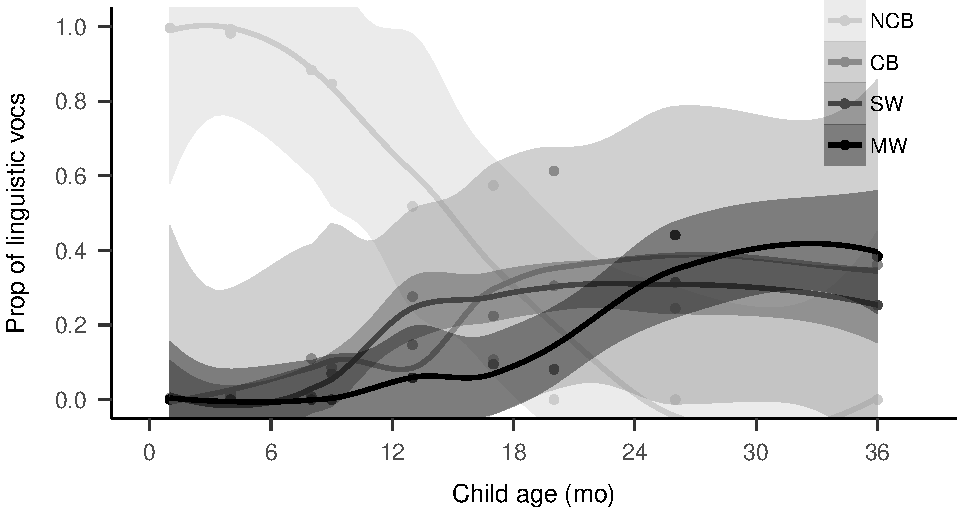
\includegraphics{Yeli-CLE_files/figure-latex/fig6-1.pdf}
\caption{\label{fig:fig6}Proportion of vocalization types used by children
across age (NCB = Non-canonical babble, CB = Canonical babble, SW =
single word utterance, MW = multi-word utterance).}
\end{figure}

\section{Acknowledgements}\label{acknowledgements}

This paper was written using the papaja library in RStudio (Aust \&
Barth, 2018).

\newpage

\section{References}\label{refs}

\begingroup
\setlength{\parindent}{-0.5in} \setlength{\leftskip}{0.5in}

\hypertarget{refs}{}
\hypertarget{ref-R-papaja}{}
Aust, F., \& Barth, M. (2018). \emph{papaja: Create APA manuscripts with
R Markdown}. Retrieved from \url{https://github.com/crsh/papaja}

\endgroup






\end{document}
